% 75-05(75쪽) — 사차함수 f(x)의 도함수 y=f'(x)(삼차·최고차항 음수)의 그래프. 스캔 화질이 낮아 TikZ 로 다시 그림.
% 원문에 있는 것만: x축 위 문자 α, β, γ(β 는 원점 왼쪽·γ 는 원점 오른쪽) · 라벨 O, x, y, y=f'(x).
% 눈금 숫자·극값 수치는 원문에 없으므로 넣지 않는다(f(α), f(β), f(γ) 의 부호를 고르는 문항이라 수치를 더하면 답이 드러난다).
% 곡선은 원문 모양 그대로 지나는 점들을 재서 smooth 로 잇는다(식이 주어진 그래프가 아니다).
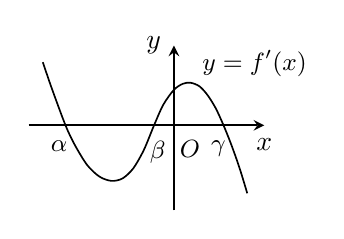
\begin{tikzpicture}[x=0.45cm, y=0.45cm, line width=0.5pt]
  \draw[->, >=stealth, line width=0.7pt] (-4.10,0) -- (2.55,0) node[below=1pt] {$x$};
  \draw[->, >=stealth, line width=0.7pt] (0,-2.40) -- (0,2.25) node[left=1pt] {$y$};
  \draw[line width=0.6pt, smooth] plot coordinates
    {(-3.70,1.78) (-3.45,1.05) (-3.06,0) (-2.80,-0.55) (-2.45,-1.12) (-2.10,-1.45)
     (-1.76,-1.57) (-1.45,-1.50) (-1.15,-1.22) (-0.85,-0.70) (-0.56,0) (-0.30,0.58)
     (0.00,1.00) (0.25,1.17) (0.47,1.20) (0.72,1.10) (0.95,0.85) (1.18,0.48)
     (1.40,0) (1.62,-0.55) (1.85,-1.20) (2.07,-1.92)};
  \node[below=2pt, font=\small] at (-3.24,0) {$\alpha$};
  \node[below=2pt, font=\small] at (-0.46,0) {$\beta$};
  \node[below=2pt, font=\small] at (0.45,0) {$\pt{O}$};
  \node[below=2pt, font=\small] at (1.26,0) {$\gamma$};
  \node[anchor=west, font=\small] at (0.52,1.74) {$y=f'(x)$};
\end{tikzpicture}
